%% LyX 2.3.6 created this file.  For more info, see http://www.lyx.org/.
%% Do not edit unless you really know what you are doing.
\documentclass[12pt,a4paper,preprint]{elsarticle}
\usepackage[latin9]{inputenc}
\usepackage{array}
\usepackage{url}
\usepackage{amstext}
\usepackage{amssymb}
\usepackage{graphicx}

\makeatletter

%%%%%%%%%%%%%%%%%%%%%%%%%%%%%% LyX specific LaTeX commands.
\special{papersize=\the\paperwidth,\the\paperheight}

\DeclareTextSymbolDefault{\textquotedbl}{T1}
%% Because html converters don't know tabularnewline
\providecommand{\tabularnewline}{\\}

%%%%%%%%%%%%%%%%%%%%%%%%%%%%%% User specified LaTeX commands.
\usepackage{amssymb}
\usepackage{lineno}
\usepackage{url}
\journal{Softwarex}

\makeatother

\usepackage{listings}
\renewcommand{\lstlistingname}{Listing}

\begin{document}
\begin{frontmatter} 

\title{GenClass: A parallel tool for data classification based on Grammatical
Evolution}

\author{Nikolaos Anastasopoulos$^{(1)}$, Ioannis G. Tsoulos$^{(2)}$, Alexandros
Tzallas$^{(2)}$}

\address{$^{(1)}$Department of Electrical and Computer Engineering, University
of Patras, Greece \\
$^{(2)}$Department of Informatics and Telecommunications, University
of Ioannina, 47100 Arta, Greece }
\begin{abstract}
A genetic programming tool is proposed here for data classification.
The tool is based on Grammatical Evolution technique and it is designed
to exploit multicore computing systems using the OpenMp library. The
tool constructs classification programs in a C -- like programming
language in order to classify the input data, producing simple if
-- else rules and upon termination the tool produces the classification
rules in C and Python files. Also, the user can use his own BNF grammar
through a command line option. The tool is tested on a wide range
of classification problems and the produced results are compared against
traditional techniques for data classification, yielding very promising
results.
\end{abstract}
\begin{keyword}
Genetic algorithm~\sep~Data classification \sep Grammatical evolution
\sep Stochastic methods
\end{keyword}
\end{frontmatter}

\linenumbers

\section{Introduction }

Data classification finds many applications on a series of practical
problems from areas such as chemistry \citep{key-1,key-2,key-7},
biology \citep{key-3,key-8}, economics \citep{key-4,key-9}, physics
\citep{key-5,key-6} etc. During the past years, many methods have
been proposed to problems of this category such as neural networks
\citep{key-10}, radial basis functions networks \citep{key-11},
support vector machines \citep{key-12}, etc. The proposed method,
which is initially described in \citep{TsoulosGenclass}, constructs
classification programs in a human readable format using the technique
of Grammatical Evolution \citep{key-13}. Grammatical evolution is
an evolutionary process that has been applied with success in many
areas such as music composition \citep{key-14}, economics \citep{key-15},
symbolic regression \citep{key-17}, robot control \citep{key-18}
and caching algorithms \citep{key-19}.

This article introduces a software tool (named GenClass) coded in
ANSI C++, for data classification using classification rules in human
readable form. The rules are created with the Grammatical evolution
method and can be applied in any classification problem, without a
priory knowledge of the dataset. Also, this tool has a series of command
line options to control the various aspects of the software, such
as mutation rate or the number of chromosomes in the genetic population.\textbf{
}Another similar software is the Parallel Program Induction (PPI)
available from the relevant URL \url{https://github.com/daaugusto/ppi},
which constructs with Grammatical Evolution programs for regression
and classification, but the PPI software has many dependencies on
other software to be compiled. Also, GenClass produces classification
problems in human readable format and it can export output in C++
and in Python. However, in the current version GenClass does not solve
regression problems. Also, recently the software NNC has been published
\citep{NNC}, which incorporates the Grammatical Evolution to construct
neural networks for regression and classification problems. Even though
the GenClass software can not be used for regression problems in the
current form it has similar execution runs as the NNC software and
also it can discover the hidden relationships between the features
of a dataset and the expected output. Also, the software GenClass
can use every core of a multicore environment and it has the ability
to load a BNF grammar from a separate input file.

The rest of this article is organized as follows: in section \ref{sec:Method-description}
the software is described in detail, in section \ref{sec:Experimental-results}
a series of experiments on some well - known classification datasets
are demonstrated, in section \ref{sec:Impact} the impact of the software
tool is discussed and finally in section \ref{conclusions} conclusions
and guidelines for further expansion of the software are presented.

\section{Software description \label{sec:Method-description}}

\subsection{The proposed algorithm }

The main steps of the algorithm are: 
\begin{enumerate}
\item \textbf{Initialization} step. 

\begin{enumerate}
\item Read the train data 
\item Set $N_{G}$ the maximum number of generations, $N_{C}$ as the number
of chromosomes, $P_{S}$ the selection rate, $P_{M}$ the mutation
rate.
\item Initialize the chromosomes of the population.
\end{enumerate}
\item \textbf{Genetic} step

\begin{enumerate}
\item \textbf{For} $i=1,\ldots,N_{g}$ \textbf{do}

\begin{enumerate}
\item Create for every chromosome in the population a classification program
using Grammatical Evolution.
\item Calculate the fitness for every chromosome of the population
\item Execute the genetic operators of selection with rate $P_{S}$ and
mutation with rate $P_{\text{}}$
\end{enumerate}
\item \textbf{EndFor}
\end{enumerate}
\item \textbf{Evaluation} step

\begin{enumerate}
\item Create a classification program for the best chromosome in the population.
\item Apply the previous program to test set and report the induced error.
\end{enumerate}
%
\end{enumerate}
The installation of the software is explained in detail in the main
page \url{https://github.com/itsoulos/GenClass/}.

\subsection{The executable genclass}

The outcome of the software compilation and installation is the executable
\texttt{genclass} under the directory \texttt{bin}. The executable
has the following command line parameters:
\begin{enumerate}
\item \texttt{-h}:The program prints a help screen.
\item \texttt{-c} \texttt{\textbf{count}}: The parameter \texttt{\textbf{count}}
determines the number of chromosomes with default value 500.
\item -f \textbf{count}. Specify fold count for fold validation. Default
value 0 (no folding). 
\item -i \textbf{grammarfile}. The string parameter \textbf{grammarfile}
stands for the user defined grammar in BNF format. If this options
is empty, then the default grammar will be used. An example of such
a file is listed in Figure \ref{fig:exampleGrammar} and it is included
under examples subdirectory of the distribution.
\item -g \textbf{gens}: The parameter \textbf{gens} determines the maximum
number of generations with default value is 200.
\item -d \textbf{count}. The parameter d determines the maximum number of
threads used by the OpenMp library. The default value is 16.
\item \texttt{-s} \texttt{\textbf{srate}}: The parameter \texttt{\textbf{srate}}
specifies the selection rate with default value 0.10 (10\%).
\item \texttt{-m} \texttt{\textbf{mrate}}: The parameter \texttt{\textbf{mrate}}
specifies the mutation rate with default value 0.05 (5\%).
\item -l \textbf{size}: The parameter \textbf{size} determines the size
of every chromosome with default value 100.
\item -p \textbf{train\_file}: The string parameter \textbf{train\_file
}specifies the file containing the points that will be used as train
data for the algorithm. The file should conform to the format outlined
in figure \ref{fig:Data-format.}. 
\item -t \textbf{test\_file}: The string parameter \textbf{test\_file }specifies
the file containing the test data for the particular problem. The
file should be in the same format as the \textbf{train\_file}.
\item -o \textbf{method}: The string parameter method specifies the output
method for the executable. The available options are

\begin{enumerate}
\item simple. The program prints output only on termination. 
\item csv. In every generation the program prints: number of generations,
train error and test error. 
\item full. The program prints in every generation detailed information
about the optimization procedure.
\end{enumerate}
\item \texttt{-r} \texttt{\textbf{seed}}: The integer parameter \texttt{\textbf{seed}}
specifies the seed for the random number generator. It can assume
any integer value.
\end{enumerate}

\subsection{The output files }

The software produces upon termination two distinct files that contains
the classification rules. The first file is written in ANSI C++ named
classifier.c and an example is shown in Figure \ref{fig:coutput}.
The second file is written in Python named classifier.py and an example
is displayed in Figure \ref{fig:pythonoutput}.

\section{Experiments \label{sec:Experimental-results}}

\subsection{A typical example }

Consider the Ionosphere dataset available from the Machine Learning
Repository. The ionosphere dataset contains data from the Johns Hopkins
Ionosphere database. The dataset has been divided into two files,
\texttt{ionosphere.train} and \texttt{ionosphere.test} under directory
\texttt{examples} of the distribution. A typical run for the \texttt{GenClass}
will be

\begin{lstlisting}
../bin/genclass -p ionosphere.train -t ionosphere.test -g 10 -o csv
\end{lstlisting}

The output of this command is shown in Figure \ref{alg:Typical-output-of}.

\subsection{Experiments}

In order to measure the efficiency of the proposed method a series
of experiments were conducted on some common classification problems
found in two major dataset databases:
\begin{enumerate}
\item UCI dataset repository, \url{https://archive.ics.uci.edu/ml/index.php}
\item Keel repository, \url{https://sci2s.ugr.es/keel/datasets.php}\citep{Keel}.
\end{enumerate}
All the experiments were conducted 30 times using different seed for
the random generator each time and averages were taken. Also, to validate
the results 10 - fold cross validation was used in all experiments.
In all experiments we have used the parameters shown in table \ref{tab:Parameters-for-the}.
The following datasets were used 
\begin{enumerate}
\item \textbf{Wine} dataset. The wine recognition dataset contains data
from wine chemical analysis.
\item \textbf{Glass} dataset. The dataset contains glass component analysis
for glass pieces that belong to 6 classes.
\item \textbf{Tae} dataset. The data consist of evaluations of teaching
performance for the University of Wisconsin-Madison.
\item \textbf{Spiral} dataset: The spiral artificial dataset contains 1000
two-dimensional examples that belong to two classes (500 examples
each). The number of the features is 2. The data in the first class
are created using the following formula: $x_{1}=0.5t\cos\left(0.08t\right),\ x_{2}=0.5t\cos\left(0.08t+\frac{\pi}{2}\right)$
and the second class data using\textbf{: $x_{1}=0.5t\cos\left(0.08t+\pi\right),\ x_{2}=0.5t\cos\left(0.08t+\frac{3\pi}{2}\right)$}
\item \textbf{Pima} dataset. The Pima Indians Diabetes dataset contains
with two categories: healthy and diabetic.
\item \textbf{Ionosphere} dataset. The ionosphere dataset (ION in the following
tables) contains data from the Johns Hopkins Ionosphere database. 
\item \textbf{Appendictis} dataset, proposed in \citep{appendicitis}.
\item \textbf{Australian}, the dataset concerns credit card applications.
\item \textbf{Hayes roth} dataset. This dataset\citep{hayesroth} contains
\textbf{5} numeric-valued attributes and 132 patterns. 
\item \textbf{Alcohol}, a dataset about Alcohol consumption \citep{Alcohol}.
\item \textbf{Dermatology}. Dataset used for differential diagnosis of erythemato-squamous
diseases. 
\item \textbf{Balance}. This data set was generated to model psychological
experimental results. 
\item \textbf{Regions2} dataset. It is created from liver biopsy images
of patients with hepatitis C \citep{regions}. 
\item \textbf{Parkinsons}. This dataset is composed of a range of biomedical
voice measurements from 31 people, 23 with Parkinson's disease (PD)\citep{parkinsons}.
\item \textbf{Wdbc}. The Wisconsin diagnostic breast cancer dataset (WDBC)
contains data for breast tumors.
\item \textbf{Popfailures}. This dataset contains records of simulation
crashes encountered during climate model.
\item \textbf{Heart}. The task is to detect the absence or presence of heart
disease.
\item \textbf{Ecoli}. The goal here is to predict the localization site
of proteins.
\item \textbf{Haberman}. A dataset about breast cancer from a study at the
University of Chicago's Billings Hospital.
\item \textbf{HouseVotes}. This data set includes votes for each of the
U.S. House of Representatives Congressmen on the 16 key votes. 
\item \textbf{Shuttle}. The task is to decide what type of control of a
spacecraft should be employed. 
\item \textbf{Lymography}. The aim here is to detect the presence of a lymphoma
in patients. 
\item \textbf{Mammographic}. This dataset be used to identify the severity
(benign or malignant) of a mammographic mass lesion.
\item \textbf{OptDigits}. Optical Recognition of Handwritten Digits data
set. 
\item \textbf{Page Blocks}. The dataset contains blocks of the page layout
of a document that has been detected by a segmentation process. 
\item \textbf{Penbased}. This is a Pen-Based Recognition of Handwritten
Digits data set.
\item \textbf{Saheart}. The dataset is about to categorize persons if have
a coronary heart disease. 
\item \textbf{Segment}. This database contains patterns from a database
of 7 outdoor images (classes). 
\item \textbf{Thyroid}. The goal in this dataset is to detect if a patient
is normal or suffers from hyperthyroidism or hypothyroidism.
\item \textbf{Eeg} datasets. As an real word example, consider an EEG dataset
described in \citep{key-20} is used here. The dataset consists of
five sets (denoted as Z, O, N, F and S) each containing 100 single-channel
EEG segments each having 23.6 sec duration. With different combinations
of these sets the produced datasets are Z\_F\_S, ZO\_NF\_S, ZONF\_S
and Z\_O\_N\_F\_S.
\end{enumerate}
The results from the experiments are displayed in Table \ref{tab:Experimental-results}.
The column Neural stands for the application of a Neural network with
10 processing nodes and the usage of a BFGS variant due to Powell
\citep{powell} as the training method. The column Mlp-Gen stands
for the application of a neural network with 10 processing nodes and
the utilization of a genetic algorithm as the training method. The
genetic algorithm used has the same parameters as in the case of GenClass
method, in order to make the results comparable. The column RBF stands
for the application of an RBF network using 10 centers. Also, the
column RBF-Gen\textbf{ }represents the application of an RBF network
with 10 processing units that is trained using a genetic algorithm
with the same set of parameters as in GenClass. Also a statistical
comparison is displayed in Figure \ref{fig:Statistical-comparison-between}.
It is evident, that the proposed method outperforms the other methods
in terms of efficiency in the majority of the objective problems.
Of course, the method could be slower than RBF or Neural network due
to the usage of Grammatical Evolution, however this increase in time
can be significantly reduced with the use of threads.  In addition,
the software appears to be slightly better in some datasets than originally
published \citep{TsoulosGenclass} due to the use of far more chromosomes
in the genetic population. 

\section{Impact\label{sec:Impact}}

This software tool produces human readable classification rules in
ANSI C++ as well as in Python format. These rules are used to classify
any classification problem without a priory knowledge about the nature
of the problem. The implemented software utilizes the Grammatical
Evolution technique to produce the classification rules based on simple
BNF grammar. The software is guided by a series of command line options
that control many critical options of the underlying method such as
the number of chromosomes, the mutation rate etc. Also, the software
is designed to be used in multi core computational environments through
the publicly available library of OpenMP. The proposed method proved
to be very reliable on a series of simple and hard classification
problems and hence the software can be used in different areas such
as physics, chemistry, medicine etc. The user needs to provide only
the patterns of the classification problem in a simple text format
and if it is required a series of command line options. Also, the
user can provide his own grammar in BNF format in a separate text
file. Finally, the software can be easily extended to be more friendly
for all users, through a graphical interface.

\section{Conclusions \label{conclusions}}

A software which implements a method for data classifications was
introduced. The method is based on grammatical evolution and the software
is designed to be portable. Future versions of the software will include 
\begin{itemize}
\item Input from various formats such as CSV, Json etc.
\item Usage of improvement stopping rules for the genetic algorithm.
\item Additional output formats. 
\end{itemize}
\begin{thebibliography}{99}
\bibitem{key-1}C. G�ler, G. D. Thyne, J. E. McCray, K.A. Turner,
Evaluation of graphical and multivariate statistical methods for classification
of water chemistry data, Hydrogeology Journal \textbf{10}, pp. 455-474,
2002

\bibitem{key-2}E. Byvatov ,U. Fechner ,J. Sadowski , G. Schneider,
Comparison of Support Vector Machine and Artificial Neural Network
Systems for Drug/Nondrug Classification, J. Chem. Inf. Comput. Sci.
\textbf{43}, pp 1882--1889, 2003.

\bibitem{key-7}Kunwar P. Singh, Ankita Basant, Amrita Malik, Gunja
Jain, Artificial neural network modeling of the river water quality---A
case study, Ecological Modelling \textbf{220}, pp. 888-895, 2009.

\bibitem{key-3}I. Guyon, J. Weston, S. Barnhill, V. Vapnik, Gene
Selection for Cancer Classification using Support Vector Machines,
Machine Learning \textbf{46}, pp. 389-422, 2002.

\bibitem{key-8}R. Marabini, J.M. Carazo, Pattern recognition and
classification of images of biological macromolecules using artificial
neural networks, Biophysical Journal \textbf{66}, pp. 1804-1814, 1994.

\bibitem{key-4}I. Kaastra, M. Boyd, Designing a neural network for
forecasting financial and economic time series, Neurocomputing \textbf{10},
pp. 215-236, 1996. 

\bibitem{key-9}Moshe Leshno, Yishay Spector, Neural network prediction
analysis: The bankruptcy case, Neurocomputing \textbf{10}, pp. 125-147,
1996.

\bibitem{key-5}S. R. Folkes,O. Lahav, S. J. Maddox, An artificial
neural network approach to the classification of galaxy spectra, Montly
Notices of the Royal Astronomical Society \textbf{283}, pp 651-665,
1996. 

\bibitem{key-6}C.Z. Cai, W.L. Wang, Y.Z. Chen, Support vector machine
classification of physical and biological datasets, Int. J. Mod. Phys.
C \textbf{14}, pp. 575, 2003

\bibitem{key-10}K. Hornik, Multilayer feedforward networks are universal
approximators, Neural Networks \textbf{2}, pp. 359-366, 1989

\bibitem{key-11}M.D. Buhmann, Radial basis functions, Cambridge monographs
on Applied and Computational Mathemetics, 2003.

\bibitem{key-12}I. Steinwart, A. Christmann, Support Vector Machines,
Information Science and Statistics, Springer, 2008.

\bibitem{TsoulosGenclass}Ioannis G. Tsoulos, Creating classification
rules using grammatical evolution, International Journal of Computational
Intelligence Studies \textbf{9}, pp. 161-171, 2020.

\bibitem{key-13}M. O\textquoteright Neill, C. Ryan, Grammatical evolution,
IEEE Trans. Evol. Comput. \textbf{5}, pp. 349--358, 2001.

\bibitem{key-14}Alfonso Ortega, Rafael S�nchez, Manuel Alfonseca
Moreno, Automatic composition of music by means of grammatical evolution,
APL '02 Proceedings of the 2002 conference on APL: array processing
languages: lore, problems, and applications Pages 148 - 155.

\bibitem{key-15}Michael O\textquoteright Neill, Anthony Brabazon,
Conor Ryan, J. J. Collins, Evolving Market Index Trading Rules Using
Grammatical Evolution, Applications of Evolutionary Computing Volume
2037 of the series Lecture Notes in Computer Science pp 343-352. 

\bibitem{key-17}M. O\textquoteright Neill, C. Ryan, Grammatical Evolution:
Evolutionary Automatic Programming in a Arbitary Language, Genetic
Programming, vol. 4, Kluwer Academic Publishers, Dordrecht, 2003

\bibitem{key-18}J.J. Collins, C. Ryan, in: Proceedings of AROB 2000,
Fifth International Symposium on Artificial Life and Robotics, 2000.

\bibitem{Keel}J. Alcal�-Fdez, A. Fernandez, J. Luengo, J. Derrac,
S. Garc�a, L. S�nchez, F. Herrera. KEEL Data-Mining Software Tool:
Data Set Repository, Integration of Algorithms and Experimental Analysis
Framework. Journal of Multiple-Valued Logic and Soft Computing 17,
pp. 255-287, 2011.

\bibitem{appendicitis}Weiss, Sholom M. and Kulikowski, Casimir A.,
Computer Systems That Learn: Classification and Prediction Methods
from Statistics, Neural Nets, Machine Learning, and Expert Systems,
Morgan Kaufmann Publishers Inc, 1991.

\bibitem{hayesroth}B. Hayes-Roth, B., F. Hayes-Roth. Concept learning
and the recognition and classification of exemplars. Journal of Verbal
Learning and Verbal Behavior \textbf{16}, pp. 321-338, 1977.

\bibitem{Alcohol}Tzimourta, Katerina D. and Tsoulos, Ioannis and
Bilero, Thanasis and Tzallas, Alexandros T. and Tsipouras, Markos
G. and Giannakeas, Nikolaos, Direct Assessment of Alcohol Consumption
in Mental State Using Brain Computer Interfaces and Grammatical Evolution,
Inventions \textbf{3}, pp. 1-12, 2018.

\bibitem{key-19}M. O\textquoteright Neill, C. Ryan, in: K. Miettinen,
M.M. Mkel, P. Neittaanmki, J. Periaux (Eds.), Evolutionary Algorithms
in Engineering and Computer Science, Jyvskyl, Finland, 1999, pp. 127--134.

\bibitem{NNC}Ioannis G. Tsoulos, Alexandros Tzallas, Dimitris Tsalikakis,
NNC: A tool based on Grammatical Evolution for data classification
and differential equation solving, Software X \textbf{10}, 2019.

\bibitem{parkinsons}Little MA, McSharry PE, Hunter EJ, Spielman J,
Ramig LO. Suitability of dysphonia measurements for telemonitoring
of Parkinson's disease. IEEE Trans Biomed Eng. 2009;56(4):1015. doi:10.1109/TBME.2008.2005954

\bibitem{regions}Giannakeas, N., Tsipouras, M.G., Tzallas, A.T.,
Kyriakidi, K., Tsianou, Z.E., Manousou, P., Hall, A., Karvounis, E.C.,
Tsianos, V., Tsianos, E. A clustering based method for collagen proportional
area extraction in liver biopsy images (2015) Proceedings of the Annual
International Conference of the IEEE Engineering in Medicine and Biology
Society, EMBS, 2015-November, art. no. 7319047, pp. 3097-3100. 

\bibitem{key-20}R.G. Andrzejak, K. Lehnertz, F. Mormann, C. Rieke,
P. David, and C. E. Elger, Indications of nonlinear deterministic
and finite-dimensional structures in time series of brain electrical
activity: Dependence on recording region and brain state, Phys. Rev.
E \textbf{64}, pp. 1-8, 2001.

\bibitem{powell}M.J.D Powell, A Tolerant Algorithm for Linearly Constrained
Optimization Calculations, Mathematical Programming \textbf{45}, pp.
547-566, 1989. 
\end{thebibliography}
\begin{figure}
\caption{Data format. The integer value D determines the dimensionality of
the problem and the value M determines the number of points in the
file. Every subsequent line contains a pattern and the final column
is the real output (category) for this pattern.\label{fig:Data-format.}}

D

M

$\begin{array}{ccccc}
x_{11} & x_{12} & \ldots & x_{1D} & y_{1}\\
x_{21} & x_{22} & \ldots & x_{2D} & y_{2}\\
\vdots & \vdots & \vdots & \vdots & \vdots\\
x_{M1} & x_{M2} & \ldots & x_{MD} & y_{M}
\end{array}$
\end{figure}
 
\begin{figure}
\caption{A typical produced C file of the tool. The double array x is the input
and the value class the estimated class of the method.\label{fig:coutput}}

\begin{lstlisting}[language=C]
#include <math.h>
int classifier(double *x)
{
     int CLASS = 0;
     if(!(x[6]<x[25]||x[4]<(((x[5]-((-5.79)/x[0]))/
        (((-503.562)/x[22])/(x[20]/x[24])))/(x[0]+(x[23]/x[4])))
        ||!(x[23]<=x[2]))) CLASS=0;         
     else CLASS=1;
     return CLASS; 
} 
\end{lstlisting}
\end{figure}
\begin{figure}
\caption{A typical output file in Python language.\label{fig:pythonoutput}}

\begin{lstlisting}[language=Python]
import ctypes 
import numpy as np from typing 
import List
def classifier(input: List):         
    fun = ctypes.CDLL("./classifier.so")         
    fun.classifier.argtypes = [ctypes.POINTER(ctypes.c_double)]         
    fun.classifier.restype = ctypes.c_int         
    a = np.array(input)         
    input_ptr = a.ctypes.data_as(ctypes.POINTER(ctypes.c_double))         
    return fun.classifier(input_ptr) 
\end{lstlisting}
\end{figure}
\begin{figure}
\caption{Typical output of the GenClass command. In every line the tool prints
the generation number, the train error as well as the test error.
At the end the tool prints the final classification rule and the estimated
train and test error.\label{alg:Typical-output-of}}

\begin{lstlisting}
 1,     15.43,     19.32     
  2,     15.43,     19.32     
  3,     15.43,     19.32     
  4,     13.71,     17.05     
  5,     12.57,     15.34     
  6,     12.57,     15.34     
  7,     12.57,     15.34     
  8,        12,     13.64     
  9,        12,     13.64 
  FINAL OUTPUT 
  EXPRESSION= 
  if(!(x7<log(cos(cos(((-788.787)+((sin(x28)/sin(cos(((-7.17)/x34))))
      +(-83.6))))))|x6>x13&x7<log(x5))) 
  CLASS=0.00  else  CLASS=1.00 
TRAIN ERROR = 12.00% 
 CLASS ERROR = 13.64% 
\end{lstlisting}
\end{figure}
\begin{figure}
\caption{An example of user defined grammar.\label{fig:exampleGrammar}}

\begin{lstlisting}
<S>::= <BEXPR>
<BEXPR>::= <XLIST><BOOLOP><EXPR>
         | !(<BEXPR>)
         | <XLIST><BOOLOP><EXPR>&<BEXPR>
         | <XLIST><BOOLOP><EXPR>|<BEXPR>
<BOOLOP>::= >
          | >=
          | <
          | <=
<EXPR>::= (<EXPR><BINARYOP><EXPR>)
        | <FUNCTION>(<EXPR>)
        | <TERMINAL>
<BINARYOP>::= +
            | -
            | *
            | /
<FUNCTION>::= sin
            | cos
            | exp
            | log
<TERMINAL>::= <XLIST>
            | <DIGITLIST>.<DIGITLIST>
            | (-<DIGITLIST>.<DIGITLIST>)
<DIGITLIST>::= <DIGIT>
             | <DIGIT><DIGIT>
             | <DIGIT><DIGIT><DIGIT>
<DIGIT>::= 0
         | 1
         | 2
         | 3
         | 4
         | 5
         | 6
         | 7
         | 8
         | 9
<XLIST>::= x1
         | x2
         | x3
         | x4
         | x5
         | x6
         | x7
         | x8
\end{lstlisting}
\end{figure}
\begin{figure}

\caption{Statistical comparison between the training methods.\label{fig:Statistical-comparison-between}}

\centering{}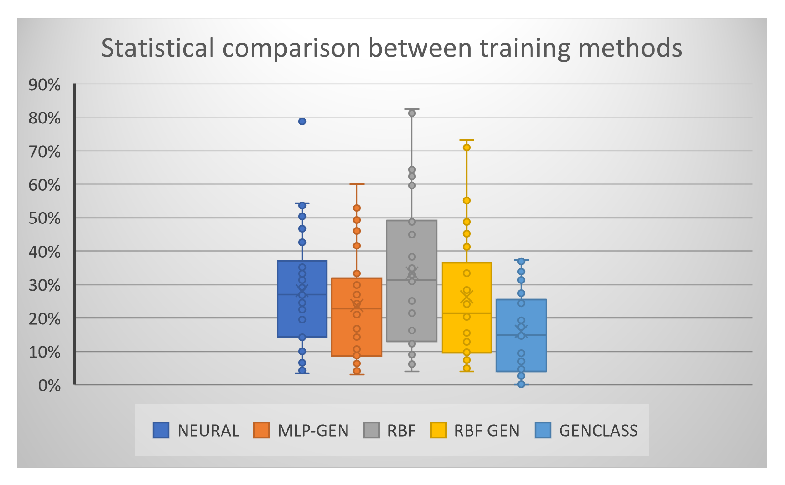
\includegraphics[scale=0.7]{statistical_genclass}
\end{figure}
\begin{table}
\caption{Parameters for the experiments.\label{tab:Parameters-for-the}}

\centering{}%
\begin{tabular}{|c|c|}
\hline 
PARAMETER & VALUE\tabularnewline
\hline 
\hline 
$N_{C}$ & 500\tabularnewline
\hline 
$N_{G}$ & 500\tabularnewline
\hline 
$P_{S}$ & $90\%$\tabularnewline
\hline 
$P_{M}$ & $5\%$\tabularnewline
\hline 
\end{tabular}
\end{table}
\begin{table}
\caption{Results.\label{tab:Experimental-results}}

\centering{}%
\begin{tabular}{|c|c|c|c|c|c|}
\hline 
DATASET & NEURAL & MLP-GEN & RBF & RBF GEN & GENCLASS\tabularnewline
\hline 
\hline 
Alcohol & 26.85\% & 25.45\% & 46.63\% & 20.29\% & 14.68\%\tabularnewline
\hline 
Appendicitis & 22.50\% & 21.30\% & 12.23\% & 11.50\% & 15.00\%\tabularnewline
\hline 
Australian & 30.48\% & 29.83\% & 34.89\% & 33.30\% & 14.57\%\tabularnewline
\hline 
Balance & 8.19\% & 8.02\% & 33.42\% & 12.96\% & 0.00\%\tabularnewline
\hline 
Dermatology & 14.33\% & 8.75\% & 62.34\% & 34.94\% & 3.72\%\tabularnewline
\hline 
Ecoli & 53.60\% & 52.86\% & 59.59\% & 56.64\% & 24.54\%\tabularnewline
\hline 
Glass & 54.24\% & 49.30\% & 50.16\% & 45.54\% & 33.81\%\tabularnewline
\hline 
Haberman & 29.94\% & 26.98\% & 25.10\% & 24.06\% & 27.33\%\tabularnewline
\hline 
Hayes Roth & 35.16\% & 33.28\% & 64.36\% & 33.54\% & 25.39\%\tabularnewline
\hline 
Heart & 25.95\% & 24.20\% & 31.20\% & 21.00\% & 17.55\%\tabularnewline
\hline 
HouseVotes & 7.54\% & 7.28\% & 6.13\% & 5.29\% & 3.72\%\tabularnewline
\hline 
Ionosphere & 15.83\% & 11.30\% & 16.22\% & 8.63\% & 8.29\%\tabularnewline
\hline 
Liverdisorder & 33.82\% & 31.37\% & 30.84\% & 28.33\% & 32.06\%\tabularnewline
\hline 
Lymography & 25.57\% & 24.55\% & 25.31\% & 20.93\% & 19.29\%\tabularnewline
\hline 
Mammographic & 27.08\% & 16.74\% & 21.38\% & 17.16\% & 17.35\%\tabularnewline
\hline 
OptDigits & 50.37\% & 45.96\% & 81.22\% & 70.93\% & 24.33\%\tabularnewline
\hline 
Page Blocks & 7.10\% & 7.06\% & 10.09\% & 9.28\% & 3.82\%\tabularnewline
\hline 
Parkinsons & 19.44\% & 14.26\% & 17.42\% & 15.47\% & 9.47\%\tabularnewline
\hline 
Penbased & 42.91\% & 41.79\% & 82.47\% & 73.16\% & 25.32\%\tabularnewline
\hline 
Pima & 29.07\% & 28.76\% & 25.78\% & 24.12\% & 25.59\%\tabularnewline
\hline 
Popfailures & 6.57\% & 6.38\% & 7.04\% & 4.95\% & 7.04\%\tabularnewline
\hline 
Regions2 & 33.32\% & 28.56\% & 38.29\% & 33.40\% & 19.52\%\tabularnewline
\hline 
Saheart & 33.22\% & 31.40\% & 32.19\% & 29.86\% & 31.30\%\tabularnewline
\hline 
Segment & 24.54\% & 21.01\% & 59.68\% & 48.70\% & 10.52\%\tabularnewline
\hline 
Shuttle & 31.29\% & 15.70\% & 32.97\% & 21.73\% & 0.15\%\tabularnewline
\hline 
Spiral & 42.60\% & 41.57\% & 44.87\% & 41.27\% & 36.90\%\tabularnewline
\hline 
Tae & 47.53\% & 47.22\% & 60.07\% & 55.07\% & 37.33\%\tabularnewline
\hline 
Thyroid & 4.28\% & 4.16\% & 10.52\% & 7.42\% & 1.89\%\tabularnewline
\hline 
Wdbc & 20.55\% & 6.76\% & 7.27\% & 6.22\% & 4.11\%\tabularnewline
\hline 
Wine & 46.63\% & 12.43\% & 31.41\% & 12.84\% & 4.71\%\tabularnewline
\hline 
Z\_F\_S & 14.17\% & 10.68\% & 13.16\% & 9.65\% & 7.00\%\tabularnewline
\hline 
Z\_O\_N\_F\_S & 78.73\% & 59.93\% & 48.71\% & 45.20\% & 32.20\%\tabularnewline
\hline 
ZO\_NF\_S & 9.97\% & 7.33\% & 9.02\% & 6.81\% & 2.60\%\tabularnewline
\hline 
ZONF\_S & 3.48\% & 3.02\% & 4.03\% & 3.98\% & 1.60\%\tabularnewline
\hline 
\end{tabular}
\end{table}


\section*{Required Metadata}

\section*{Current code version}

\begin{table}[!h]
\begin{tabular}{|l|p{6.5cm}|p{6.5cm}|}
\hline 
\textbf{Nr.}  & \textbf{Code metadata description}  & \tabularnewline
\hline 
C1  & Current code version  & 1.0 \tabularnewline
\hline 
C2  & Permanent link to code/repository used for this code version  & \url{https://github.com/itsoulos/GenClass/} \tabularnewline
\hline 
C3  & Legal Code License  & GNU General Public License (GPL) \tabularnewline
\hline 
C4  & Code versioning system used  & git \tabularnewline
\hline 
C5  & Software code languages, tools, and services used  & C++\tabularnewline
\hline 
C6  & Compilation requirements, operating environments \& dependencies  & Linux \tabularnewline
\hline 
C7  & If available Link to developer documentation/manual  & \url{https://github.com/itsoulos/GenClass/wiki}\tabularnewline
\hline 
C8  & Support email for questions  & itsoulos@uoi.gr\tabularnewline
\hline 
\end{tabular}
\end{table}

\end{document}
